% ltex: language=it
\chapter{Data Flow Diagram}\label{chap:data_flow_diagram} % (fold)
I \textbf{\ac{dfd}} traggono origine dalla teoria dei grafi e sono stati utilizzati anche precedentemente all'avvento dei computer per la gestione delle informazioni.
Sono stati impiegati per la prima volta, nel settore dell'ingegneria del software, solo verso la metà degli anni 70.
\begin{quote}
    Non esiste in letteratura tutt'oggi una definizione universalmente accettata e sono presenti molteplici differenti formulazioni operative.
\end{quote}
%
\section{Cosa modella un DFD?}\label{sec:cosa_modella_un_dfd} % (fold)
Un sistema è visto come una \textbf{rete di processi funzionali} interconnessi da \textbf{depositi di dati}.
I \ac{dfd} enfatizzano le operazioni effettuate sulle informazioni e le dipendenze funzionali che vengono a crearsi fra i vari processi in base ai flussi di informazione.
\\
I processi possono essere definiti a qualunque livello di astrazione, raffinabili mediante \red{scomposizione gerarchica} in un insieme di processi più elementari.
% section Cosa modella un DFD? (end)
%
\section{Entità rappresentate}\label{sec:dfd_entita_rappresentate} % (fold)
\noindent
\begin{minipage}{0.2\textwidth}
    \centering
    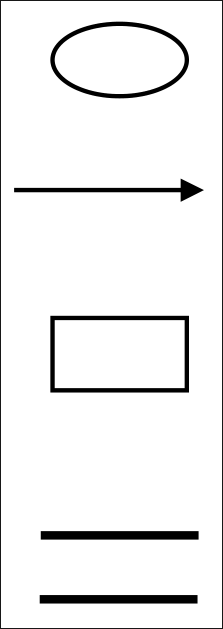
\includegraphics[width=0.5\textwidth]{assets/entita-dfd-dyntax.png}
\end{minipage}
\hfill
\begin{minipage}{0.79\textwidth}
    \begin{itemize}
        \item \textbf{processo}, detti anche \textbf{bolle}, che trasformano i dati;
        \item \textbf{flussi}, che muovono i dati;
        \item \textbf{agenti esterni}, detti anche \textbf{terminatori}, che producono e consumano i dati;
        \item \textbf{depositi di dati}, che memorizzano le informazioni in modo passivo;
    \end{itemize}
\end{minipage}
\subsection{Sintassi}\label{sub:dfd_sintassi} % (fold)
Un \ac{dfd} è una quartupla $<P,\,D,\,A,\,F>$ dove:
\begin{itemize}
    \item $P = \pg{\vc{p_1}{p_n}}$ è un insieme finito, non vuoto, di processi;
    \item $D = \pg{\vc{d_1}{d_r}}$ è un insieme finito di depositi;
    \item $A = \pg{\vc{a_1}{a_s}}$ è un insieme finito di agenti;
    \item $F = \pg{ f \in \pt{P\times \pt{P \cup D \cup A}} \cup \pt{\pt{P\cup D\cup A} \times P}}$ è un insieme finito di flussi;
\end{itemize}
% subsection Sintassi (end)
%
\subsection{Rappresentazione}\label{sub:dfd_rappresentazione} % (fold)
Un \ac{dfd} si rappresenta tramite un grafo orientato in cui ogni nodo appartiene a uno dei tre sistemi $P$, $D$ o $A$, e ogni arco orientato rappresenta un flusso di dati.
\begin{cimage}
   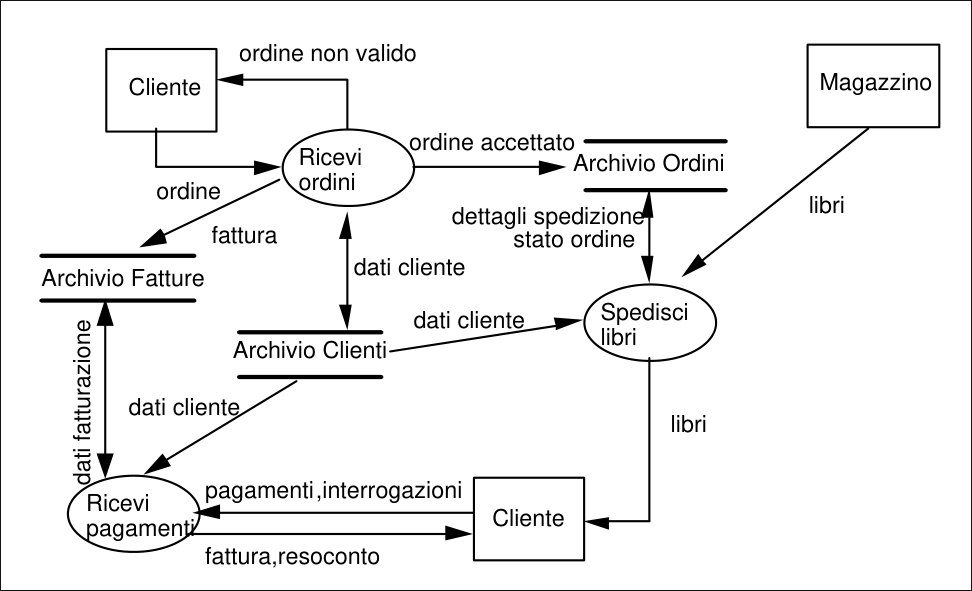
\includegraphics[width=.6\textwidth]{assets/rapp-dfd-es-visual.png}
   \caption{Un DFD che descrive i rapporti fra una libreria e i suoi clienti}\label{fig:rapp-dfd-es-visual}
\end{cimage}
\begin{tip}
    \begin{itemize}
        \item nomi univoci per identificare processi, flussi di dati, agenti e depositi;
        \item non si rappresentano le eccezioni e il trattamento degli errori, rimandando questi dettagli alle fasi dell'analisi;
        \item un \ac{dfd} non è un diagramma di flusso, dove le frecce indicano un ordinamento negli eventi;
        \item in alcune estensioni, come nella notazione OMT è possibile rappresentare anche flussi di controllo.
            Anticiparli in un \ac{dfd} comporta di fatto una duplicazione se si usa anche un modello dinamico;
    \end{itemize}
\end{tip}
\begin{warning}[Regole]
    \begin{itemize}
        \item scegliere nomi significativi per i processi, flussi, depositi e agenti;
        \item numerare i processi;
        \item disegnare i \ac{dfd} seguendo criteri estetici;
        \item evitare \ac{dfd} eccessivamente complessi;
        \item accertarsi della coerenza interna di un \ac{dfd} e che sia coerente con quelli a esso associati;
        \item esiste una convenzione spesso accettata in molte versioni: un flusso da o verso un \textbf{deposito} possa essere \textbf{non etichettato} quando i dati trasferiti corrispondono a \textbf{un oggetto (record) interno}.
    \end{itemize}
\end{warning}
\begin{critical}[Vincoli]
    \begin{itemize}
        \item evitare processi a consumo infinito (pozzi);
        \item sospettare di processi a generazione spontanea;
        \item depositi a sola lettura o a sola scrittura sono rari;
        \item non devono esistere flussi di dati fra:
            \begin{itemize}
                \item due agenti esterni;
                \item due depositi;
                \item un'entità esterna e un deposito;
            \end{itemize}
    \end{itemize}
\end{critical}
\begin{cimage}
    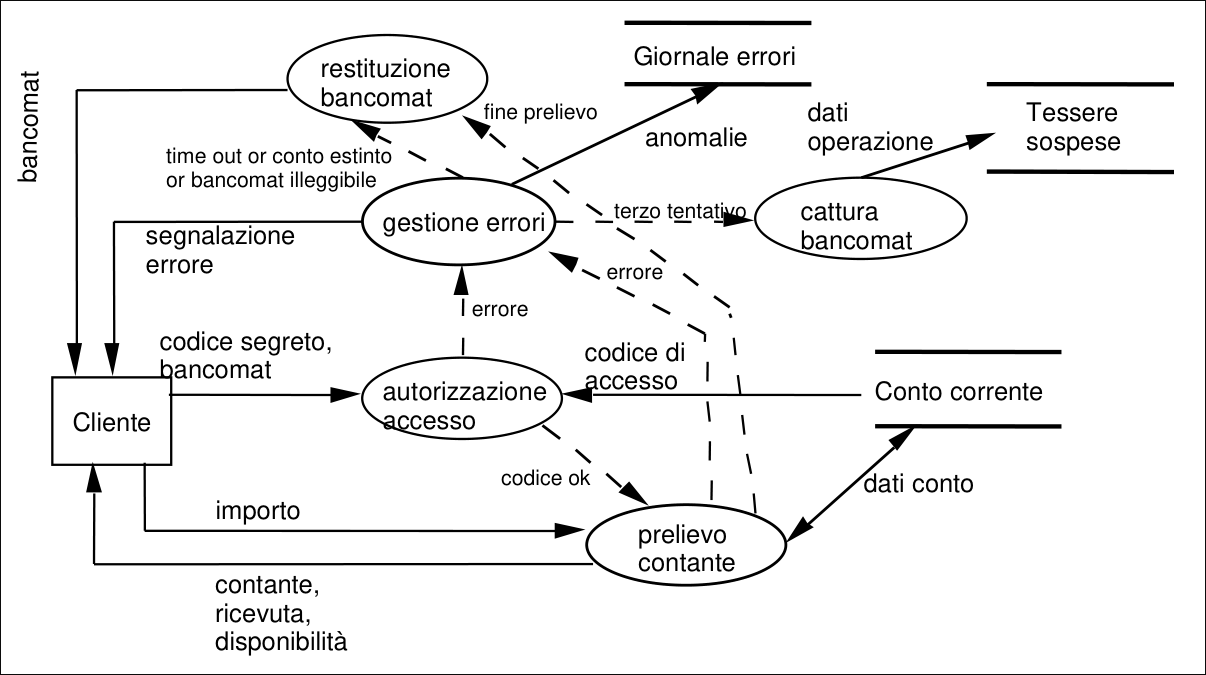
\includegraphics[width=.6\textwidth]{assets/dfd-flussi-es-visual.png}
    \caption{Un DFD con i flussi di controllo}\label{fig:dfd-flussi-es-visual}
\end{cimage}
%
\paragraph{Consigli pratici}\label{par:dfd_consigli_pratici} % (fold)
\begin{enumerate}
    \item Evitare di costruire \ac{dfd} molto sbilanciati:
        \begin{itemize}
            \item se in un \ac{dfd} compaiono bolle atomiche e bolle che richiedono successivi livelli di dettaglio ciò è sintomo di trascuratezza nel modellare il sistema;
        \end{itemize}
    \item Prestare attenzione al problema della presentazione dei \ac{dfd}:
        \begin{itemize}
            \item può essere molto utile affiancare a documenti cartacei strumenti di visualizzazione che consentano di navigare la gerarchia mostrandone viste a vari livelli di astrazione;
        \end{itemize}
    \item Verificare che i \ac{dfd} siano fra loro coerenti:
        \begin{itemize}
            \item al fine di garantire che ciascun \ac{dfd} sia coerente con il \ac{dfd} genitore si verifica che i flussi di dati relativi a una bolla a un livello corrispondente ai flussi di dati evidenziati nel \ac{dfd} che esplode quella bolla;
        \end{itemize}
    \item Mostrare un deposito al livello più alto di astrazione, quando se ne scopre la necessità come interfaccia fra due o più processi, quindi riportare il deposito in ogni diagramma di livello inferiore che descrive quei processi;
    \item Verificare che un agente esterno collegato a un processo in certo livello compaia e resti connesso a un discendente di quel processo nel livello gerarchico inferiore;
\end{enumerate}
% paragraph Consigli pratici (end)
%
\paragraph{Strategie per la costruzione}\label{par:dfd_strategie_per_la_costruzione} % (fold)
\begin{description}
    \item[top-down] Decomposizione di un processo in una serie di sottoprocessi chiaramente identificabili e indipendenti
    \item[bottom-up] A partire da una collezione di concetti elementari si costruivano via via le connessioni fra essi
    \item[mixed] Raffinamento di un \ac{dfd} di massima in stadi successivi con tecniche top-down e bottom-up
    \item[outside-in] Parte delle interfacce con il sistema e propaga in avanti gli ingressi evidenziando i processi coinvolti nei flussi di dati o propaga all'indietro le uscite
\end{description}
% paragraph Strategie per la costruzione (end)
% subsection Rappresentazione (end)
% section Entità rappresentate (end)
% chapter Data Flow Diagram (end)
